\chapter{Bivariate Analysis}
\label{ch:bivariate-analysis}

In previous chapters, we examined one variable at a time. In this chapter we will study the \emph{relationship}\index{relationship} (also: \emph{correlation}\index{correlation} or \emph{association}\index{association}) between variables. We speak of a relationship between two variables when the value of one variable systematically changes depending on the value of the other. In other words, it determines to what extent it becomes easier to predict the value of one variable based on the value of the other variable.

\section{Learning Goals}
\label{sec:bivariate-analysis-learning-goals}

By the end of this chapter you must be able to:

\begin{itemize}
    \item Explain the following concepts:
    \begin{itemize}
        \item dependent variable, independent variable;
        \item a relationship (correlation, association) between two variables, ascending/descending relationship, linear relationship;
    \end{itemize}
    \item Identify suitable analysis techniques for the combinations of measurement levels discussed in this chapter;
    \item For a combination of two qualitative variables:
    \begin{itemize}
        \item Create a cross table and apply Cochran's rule;
        \item Calculate the $\chi^2$ statistic;
        \item Apply the $\chi^2$-test (for association and goodness-of-fit);
        \item Calculate and interpret standardized residuals;
        \item Calculate the value of Cramér's V and interpret the result
    \end{itemize}
    \item For a combination of a qualitative independent and a quantitative dependent variable:
    \begin{itemize}
        \item Apply the correct variant of the $t$-test for two samples (paired, independent);
        \item Calculate the effect size (Cohen's $d$) and interpret the result;
    \end{itemize}
    \item For a combination of two quantitative variables:
    \begin{itemize}
        \item determine the equation of the regression line and plot it;
        \item calculate the covariance, the correlation coefficient and the coefficient of determination and describe the value using the correct terms;
    \end{itemize}
    \item Identify and apply appropriate visualization techniques for the combinations of measurement levels discussed in this chapter;
    \item Interpret a given graph consisting of two variables, a.o.~naming the graph type, deducing whether there is a relationship, what type of relationship and the correlation (weak, moderate, strong).
    \item Explain, based on a given situation, that correlation does not imply a causal relationship, and why;
\end{itemize}

\section{Inleiding}
\label{sec:analyse2var-inleiding}

When describing a relationship between variables, we make a distinction between:

\begin{itemize}
    \item The \emph{dependent variable}\index{variable!dependent}, for which we want to predict the value;
    \item The \emph{independent variable}\index{variable!independent}, for which we know the value and use this value to make a prediction.
\end{itemize}

So if the value of the independent variable changes in a certain way, we expect the value of the dependent variable to change in a predictable way.

\begin{example}
    An example in which relationships can be found between variables is Ant Colony Optimization (ACO), a technique used in various computational problems. The technique is based on how ants search for, and find food, and how they communicate this to the group. Ants spread pheromones when they go out looking for food. The longer the path, the less pheromones the path will contain, the shorter the path, the more likely a large concentration of pheromones can be found. Other ants are attracted by these pheromones and will therefore follow the most traveled paths to get to a particular food source. We can now research whether the time required for finding a path has a relationship with one of the following variables:
    
    \begin{itemize}
        \item The extent to which pheromones are distributed
        \item The degree to which a pheromone disappears
        \item The number of obstacles between the ant nest and the food source
        \item The shape of the obstacles between the nest and source (e.g. do ants find a path faster if the obstacles have no corners)
    \end{itemize}
\end{example}

To investigate whether there is a relationship between two variables, different analysis and visualization techniques can be used, depending on the measurement level. Table~\ref{tab:bivariate_analysis} provides an overview of suitable analysis techniques discussed in this syllabus, and Table~\ref{tab:bivariate_visualization} of suitable graph types.

However, note that there are many other analysis techniques that are not discussed in this syllabus! This syllabus only provides a sneak preview\ldots If later during your career, you need to use statistical techniques (the authors of this syllabus strongly believe that this can happen effectively), we recommend spending some time researching wether there exist better techniques for your specific research question.

\begin{table}
    \begin{tabular}{llll}
        \toprule
        \textbf{Independent}    & \textbf{Dependent}    & \textbf{Test}                 & \textbf{Metric}         \\
        \midrule
        Qualitative             & Qualitative           & $\chi^2$-test                 & Cramér's $V$            \\
        Qualitative             & Quantitative          & two-sample $t$-test           & Cohen's $d$             \\
        Quantitative            & Quantitative          & ---                           & Regression, correlation \\
        \bottomrule
    \end{tabular}
    \caption{Overview of techniques for analysing the relationship between two variables. The table provides the suitable statistical tests, and the metrics that can be used to express the relationship.}
    \label{tab:bivariate_analysis}
\end{table}

\begin{table}
    \begin{tabular}{lll}
        \toprule
        \textbf{Independent}    & \textbf{Dependent}    & \textbf{Graph Type}                                  \\
        \midrule
        Qualitative             & Qualitative           & Mosaic plot, horizontal stacked bar chart, clustered bar chart \\
        Qualitative             & Quantitative          & Boxplot, bar chart with error bars                  \\
        Quantitative            & Quantitative          & Scatter plot, regression line                    \\
        \bottomrule
    \end{tabular}
    \caption{Overview of techniques for visualizing the relationship between two variables.}
    \label{tab:bivariate_visualization}
\end{table}

\section{Qualitative--Qualitative}
\label{sec:qualitative-qualitative}

In this section we investigate methods for researching the relationship between two qualitative variables. All methods are based on a summarizing table of frequencies of the variables, the cross table (cfr. Section~\ref{ssec:cross-tables}). Based on this, a statistic is calculated that expresses how great the differences are between the two variables, the so-called ``Chi-squared'', notation $\chi^2$\footnote{Chi, $\chi$ is a letter from the Greek alphabet.} (cfr. Section~\ref{ssec:chi-square}). The $\chi^2$-test (cfr. Section~\ref{ssec:test-of-independence} and Section~\ref{ssec:goodness-of-fit-test}) can be used to determine wether the value of $\chi^2$ indicates that there is a relationship between the two variables. There is also another technique, Cramér's $V$ (cfr. Section~\ref{ssec:cramers-v}), which reduces the value of $\chi^2$ to a number between 0 and 1, and can be used to derive the strength of the relationship.

\subsection{Cross Tables}
\label{ssec:cross-tables}

\begin{definition}[Cross Table]
    A cross table\index{cross table}\index{table!cross} (also called contingency table\index{table!contingency}, cross tabulation or crosstab) summarizes the frequencies of two variables.
    
    Each cell of the last column contains the sum of the corresponding row, and each cell of the last row contains the sum of the corresponding column. These values are called the \emph{marginal totals}\index{total!marginal}\index{marginal total}.
\end{definition}

\begin{table} \centering
    \begin{tabular}{@{}rrrr}
        \toprule
              & Women & Men &  Total \\
        \midrule
         Good &     9 &   8 &     17 \\
   Sufficient &     8 &  10 &     18 \\
 Insufficient &     5 &   5 &     10 \\
          Bad &     0 &   4 &      4 \\
        Total &    22 &  27 &     49 \\
        \bottomrule
    \end{tabular}
    \caption{A cross table for the appreciation by men and women of a particular range of products.}
    \label{tab:crosstable0}
\end{table}

How can we determine, based on a cross table, whether there is a relationship between two variables? For example, take a look at the crosstable of Table~\ref{tab:crosstable0}. This table summarizes the results of a survey in which 49 persons (22 woman and 27 men) were asked to give a rating (good, sufficient, bad) for a particular range of products. If there is a relationship between the two variables, namely the gender (independent) and the rating (dependent), we should be able to see that women and men gave fundamentally different ratings. On the other hand, if the proportions of the different ratings are (approximately) the same for both women and men, there is \emph{no} relationship.

An ordinary cross table cannot be directly used for drawing conclusions, as analyzing a possible coherence between variables is not straightforward based on absolute frequencies. After all, there are more men than women in the survey! Instead, we have to calculate the percentages, i.e.~within each column we need to calculate how often each rating occurs \emph{in proportion}. The sum of all percentages in a column needs to be equal to 100\%. A quick review of the rules regarding calculating percentages:

\begin{itemize}
  \item To determine what percent $x$ is of $y$, divide $x$ by $y$ and multiply by 100: $p = \frac{x}{y} \times 100$. For example: what percentage is 15 of 20? $\frac{15}{20} \times 100 = 75$, so 75\%.
  \item To calculate $x\%$ of $y$: $\frac{x \times y}{100}$. For example: calculate 60\% of 30? $\frac{60 \times 30}{100} = 18$.
\end{itemize}

Table~\ref{tab:crosstable1} provides an overview of the percentages per gender for each appreciation that occured in the sample. For example, we see that 41\% of women gave a good rating (because 9 is approximately 41\% of 22), compared to 30\% of men.

\begin{table} \centering
  \begin{tabular}{@{}rrrrrrr@{}}
  	\toprule
                & Women & Men &  Total & Women \% & Men\% & Total  \\
  	\midrule
  	       Good &     9 &   8 &     17 &     41\% &  30\% &   35\% \\
     Sufficient &     8 &  10 &     18 &     36\% &  37\% &   37\% \\
   Insufficient &     5 &   5 &     10 &     23\% &  18\% &   20\% \\
            Bad &     0 &   4 &      4 &      0\% &  15\% &    8\% \\
  	      Total &    22 &  27 &     49 &    100\% & 100\% &  100\% \\
  	\bottomrule
  \end{tabular}
  \caption{The crosstable, including percentages of the different values.}
  \label{tab:crosstable1}
\end{table}

We can now ask ourselves whether the choice of rating depends on the gender of the repondent. There are differences between the two columns, se you could suspect that this is indeed the case. Smaller differences indicate a weak relationship, whereas greater differences indicate a stronger coherence.

\subsection{\texorpdfstring{$\chi^{2}$}{chi-square}}
\label{ssec:chi-square}

The previous section indicates the need for a measure to express the difference between the ratios in both columns. One way to express this is the so-called \emph{chi-square} statistic (notation: $\chi^{2}$). The value of $\chi^2$ equals 0 when there is no difference between the proportions in the columns of a crosstable, and therefore when there is absolutely no coherence between the variables. If there is a difference, $\chi^2$ will be a positive number. The larger the value, the greater the mutual differences between both columns, and the stronger the relationship.

The procedure for calculating the value of $\chi^2$ based on a crosstable is as follows:

\begin{enumerate}
  \item First, create a crosstable containing the marginal totals (cfr. Table.\ref{tab:crosstable0}).
  \item Next, calculate the so-called \emph{expected frequency} of each cell (notation: $e$). This is the absolute frequency you would \emph{expect} if you assume there is no relationship at all between the variables. You can calculate the expected frequency as follows:
  
  \begin{equation}
      e = \frac{row total \times column total}{n}
  \end{equation}

  with:

  \begin{itemize}
      \item $row total$ the sum of all values of the cell's row
      \item $column total$ the sum of all values of the cell's column
      \item $n$ the number of observations
  \end{itemize}

  For cell$_{1,2}$ (the expected number of man that answered ``good'') this corresponds to $\frac{17 \times 27}{49} \approx 9.37\%$.

  \item Next you calculate the difference between the \emph{observed} (notation: $o$) and the \emph{expected} frequency ($e$). (cfr. Table~\ref{tab:crosstable2}).

  \begin{table} \centering
    \begin{tabular}{@{}rrrrrrr@{}}
      \toprule
                &                       Women &                          Men &  Total & Women \% &   Men\% &   Total \\
      \midrule
           Good &  $9 -\textcolor{red}{7.63}$ &  $8 - \textcolor{red}{9.36}$ &   $17$ &   $41$\% &  $30$\% &  $35$\% \\
     Sufficient & $8 - \textcolor{red}{8.08}$ & $10 - \textcolor{red}{9.91}$ &   $18$ &   $36$\% &  $37$\% &  $37$\% \\
   Insufficient & $5 - \textcolor{red}{4.48}$ &  $5 - \textcolor{red}{5.51}$ &   $10$ &   $23$\% &  $18$\% &  $20$\% \\
            Bad & $0 - \textcolor{red}{1.79}$ &  $4 - \textcolor{red}{2.20}$ &    $4$ &    $0$\% &  $15$\% &   $8$\% \\
          Total &                        $22$ &                         $27$ &   $49$ &  $100$\% & $100$\% & $100$\% \\
    \bottomrule
    \end{tabular}
    \caption{The crosstable, with the expected frequency $e$ (indicated in red) subtracted from the observed frequency $o$ for each cell.}
    \label{tab:crosstable2}
  \end{table}

  \item The final step involves calculating a measure for the dispersion of each cell. Similar to calculating the variance of a sample (cfr. Section~\ref{ssec:variance-and-standard-deviation}), we calculate the squared difference so that the result is always positive and larger deviations will have a greater influence in the result.

  We will also divide the dispersion by the expected frequency to make them both relatively equally important. For example: a standard deviation of 5 for an expected frequency of 20 is bigger than for an expected frequency of 200. The resulting equation for each cell of the crosstable is (cfr. Table~\ref{tab:crosstable3}):

  \begin{equation}
    \frac{(o - e)^{2}}{e}
  \end{equation}

  \begin{table} \centering
    \begin{tabular}{@{}rrrrrrr@{}}
      \toprule
                &                    Women &                      Men &  Total & Women \% &   Men\% &   Total \\
    	\midrule
           Good & $\textcolor{blue}{0.24}$ & $\textcolor{blue}{0.20}$ &   $17$ &   $41$\% &  $30$\% &  $35$\% \\
     Sufficient & $\textcolor{blue}{0.00}$ & $\textcolor{blue}{0.00}$ &   $18$ &   $36$\% &  $37$\% &  $37$\% \\
   Insufficient & $\textcolor{blue}{0.06}$ & $\textcolor{blue}{0.05}$ &   $10$ &   $23$\% &  $18$\% &  $20$\% \\
            Bad & $\textcolor{blue}{1.80}$ & $\textcolor{blue}{1.46}$ &    $4$ &    $0$\% &  $15$\% &   $8$\% \\
          Total &                     $22$ &                     $27$ &   $49$ &  $100$\% & $100$\% & $100$\% \\
    	\bottomrule
    \end{tabular}
    \caption{The crosstable, with the squared difference divided by the expected frequency, $\frac{(o - e)^2}{e}$ (in blue). Note that these values are rounded to two decimal places, so we lose some of the precision.}
    \label{tab:crosstable3}
  \end{table}

  \item Finally, we take the sum of all values to determine the value of $\chi^{2}$:
  \item 
  \begin{equation}
    \chi^{2} = \sum \frac{(o - e)^{2}}{e}
    \end{equation}
    
    In our example: $\chi^2 \approx 3.8105$.
\end{enumerate}

However, this value $\chi^2 \approx 3,8105$ itself \emph{still} does not say much. Under what conditions can we say whether there is a relationship between the two variables? And how strong is this relationship? This will also depend on the size of the table and the total number of observations. In a crosstable consisting of more rows/columns, the value of $\chi^2$ will have to be larger to conclude that there is a relationship.

\subsection[Chi-squared Distribution]{$\chi^{2}$-distribution}
\label{ssec:chi-squared-distribution}

In Section~\ref{ssec:test-of-independence} we will introduce the $\chi^2$-test. This test uses the so-called $\chi^2$-distribution for determining the probability value or critical value. Although $\chi^2$-distribution does not occur in nature, and therefore few phenomenoms can be modeled using this distribution, it is \emph{very} useful in this \emph{context}.

Assume that  $X_{1}, X_{2}, \dots X_{v}$ are independent variables with a standard normal distribution ($\sim N(0,1)$). The $\chi^{2}$ (chi-square) variable is then defined as follows:

\[ \chi^{2}_{v} = X_{1}^{2} + X_{2}^{2} + \dots + X_{v}^{2} \]

The value of $v$ is the number of degrees of freedom of the variable. $\chi^{2}$ is a continuous random variable, and has a positive value because it is calculated by taking the sum of the squared differences. The distribution function is as follows:

\[ f_{n}(x) = \frac{1}{2^{\frac{n}{2}}\Gamma(\frac{n}{2})} x^{\frac{n}{2} -1} e^{\frac{x}{2}} \]

The expected value (= mean) is $v$ with a variance $2v$. The mode of $v \geq 2$ is $v-2$.

To determine the necessary values within the $\chi^{2}$-distribution (e.g. right-tailed probability, critical value), we can either use a table \footnote{For example \url{https://people.richland.edu/james/lecture/m170/tbl-chi.html}}, or statistical software such as R.

\begin{figure}
  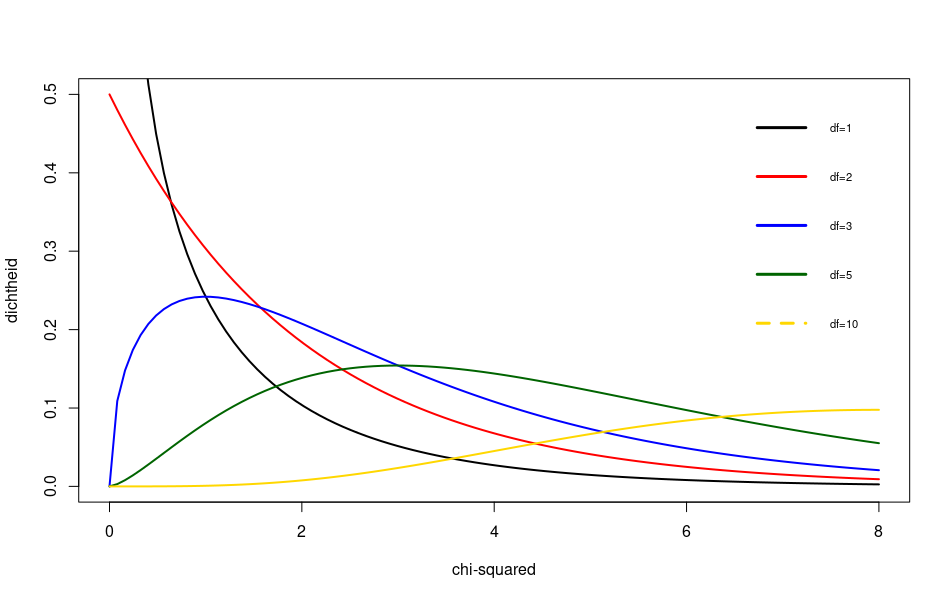
\includegraphics[width=\textwidth]{chi-squared-distribution}
  \caption{Density function of the$\chi^2$-distribution for different degrees of freedom $df$.}
  \label{fig:chi-squared-distribution}
\end{figure}

\subsection{Test of Independence}
\label{ssec:test-of-independence}

A test of independence\index{test of independence} is used to determine if there is a relationship between two qualitative variables by using the $\chi^2$ statistic. This test is also called the $\chi^2$-test\index{$\chi^2$-test}\index{test!$\chi^2$-} of association, or the $\chi^2$ crosstable test, and was developed by the English mathematician and statistician Karl Pearson\index{Pearson!Karl}.

\subsubsection{Testing Procedure}

The testing procedure is as follows:

\begin{enumerate}
  \item \textbf{Formulate both hypotheses}
  As a null hypothesis, we state that there is no relationship between the independent and the dependent variable (so we expect a small value for $\chi^2$).
  As alternative hypothesis, we state that there \emph{is} a relationship (and therefore we expect $\chi^2$ to be large).
  \begin{itemize}
    \item $H_{0}$: There is no relationship between the variables (or: the variables are independent)
    \item $H_{1}$: There is a relationship between the variables
  \end{itemize}

  \item \textbf{Determine significance level $\alpha$}
  
  \item \textbf{Calculate the value of the test statistic in the sample}
  \[ \chi^{2} = \sum_{i} \frac{(o_{i} - e_{i})^{2}}{e_{i}} \]

  \item The value of $\chi^2$ follows the $\chi^2$-distribution (cfr. Section~\ref{ssec:chi-squared-distribution}). This stochastic distribution has an additional parameter, the number of degrees of freedom $df$. For a crosstable test, $df = (r - 1) \times (k - 1)$ with $r$ the number of rows and $k$ the number of columns.

  Using this distribution, we can draw a conclusion in two equivalent ways:
  \begin{enumerate}
    \item \textbf{Calculate and plot the critical area}. The critical value $g$ is the value for which $P(\chi^2 > g) = \alpha$. This test is always right-tailed. If $\chi^2 < g$, we are inside the \emph{region of acceptance}, and we cannot reject the null hypothesis. If $\chi^2 > g$, we are inside the \emph{region of rejectance} or \emph{critical region} and we will reject the null hypothesis.
    \item \textbf{Calculate the probability value $p$}. This is the right-tail probability for the $\chi^2$ statistic in the sample, depending on the number of degrees of freedom. The interpration of the $p$-value is ``If we assume that there is \emph{no} relationship between the two variables, what is the probability of obtaining a value for $\chi^2$ in a sample that is as least as large as the obtained one?'' If $p > \alpha$ (and therefore there is a relatively great probability to obtain this $\chi^2$-value), we accept the null hypothesis, if $p < \alpha$, we reject it.
  \end{enumerate}

  \item Finally, we formulate the conclusion and answer the research question.
\end{enumerate}  

Applied to the previous example:

\begin{enumerate}
  \item \textbf{Formulate both hypotheses:}
  \begin{itemize}
    \item $H_0$ There is no relationship between gender and rating
    \item $H_1$ There is a relationship between gender and rating
  \end{itemize}
  \item \textbf{Determine significance level:} $\alpha = 0.05$
  
  \item \textbf{Calculate the value of the test statistic in the sample}
  
  $\chi^2 \approx 3.8105$ (cfr. Section~\ref{ssec:chi-square})
  
  \item Determine the number of degrees of freedom $df = (r - 1) \times (k - 1) = (4 - 1) \times (2 - 1) = 3$.
  
  \begin{enumerate}
    \item \textbf{Calculate the critical value:} $g \approx 7.815$. In this case $\chi^2 < g$, so we are inside the region of acceptance. Therefore we cannot reject $H_0$.
    \item \textbf{Calculate the probability value:} $p \approx 0.2827$. There is a probability of around 28\% to obtain this $\chi^2$-value from a sample. That is quite large, certainly larger than $\alpha$. As a result we cannot reject $H_0$.
  \end{enumerate}

  \item We can therefore assume that, based on this sample, there is no reason to assume that there is a relationship between gender and rating. In other words, there are no significant differences between the ratings given by women and men.
\end{enumerate}


We investigate another example of the test of independence based on a study by \textcite{Doll1954} regarding the relationship between smoking and cancer. In 1951, Doll and Hill wrote to all British general practitioners (GPs) requesting information about their age and smoking behavior. Next, they tracked death reports and cause of death over years and repeated this periodically. The first results, after around four years, are summarized in Table~\ref{tab:dollhill}. It can easily be concluded from this table that there is no relationship between smoking and lung cancer. In (over) four years, only $(84 / 24354) * 100 = 0.35\%$ of British GPs died of lung cancer, and this with only $(83 / 21261) * 100 = 0.39\%$ of smokers among them. This result is small, but it is much larger than the result for the non-smokers $(1 / 3093) * 100 = 0,032\%$.

\begin{table}
  \begin{center}
    \begin{tabular}{@{}lllll@{}}
    	\toprule
    	                & \textbf{Lung Cancer} & \textbf{No} & \textbf{Yes} & \textbf{Total} \\
    	\midrule
    	\textbf{Smoker} & \textbf{Yes}         & 21178       & 83           & 21261           \\
    	                & \textbf{No}          & 3092        & 1            & 3093            \\
    	                & \textbf{Total}       & 24270       & 84           & 24354           \\
    	\bottomrule
    \end{tabular}
  \end{center}
  \caption{Results of the research of~\textcite{Doll1954}}
  \label{tab:dollhill}
\end{table}

The table illustrates thate there is a significant difference between the observed number of smokers that died of lung cancer and the expected frequencies in this cell. The same applies to the small number of GPs who do not smoke, but who have died of lung cancer. This observation makes us suspicious whether the earlier tentative conclusion is correct. We can deal with this uncertainty by calculating the test statistic $\chi^{2}$. We do this in the familiar way:

\begin{enumerate}
  \item \textbf{Formulate both hypotheses:}
  \begin{itemize}
    \item $H_{0}$: There is no relationship between smoking and dying from lung cancer
    \item $H_{1}$: There is a relationship between smoking and dying from lung cancer
  \end{itemize}
  \item \textbf{Determine $\alpha$ and $n$:} $\alpha = 0.05$ and $n = 24354$.
  \item \textbf{Calculate the value of the test statistic in the sample}:
  \[ \chi^{2} = \sum_{i=1}^{k \times r} \frac{(o_{i} - e_{i})^{2}}{e_{i}} \approx 10.071 \]
  \item \textbf{Calculate and plot the critical area}: The number of degrees of freedom is $df = (r-1)(k-1) = 1$, so for the selected significance level the critical value is 3.8415. Our test statistic is inside the critical region so we reject $H_{0}$.
\end{enumerate}

We must therefore reject $H_{0}$, which states that there is no relationship between the two variables, in favor of $H_{1}$, which states that there is a relationship between the two variables: smokers are more likely to die of lung cancer compared to non-smokers.

But, is this evidence that smoking \emph{causes} lung cancer, as is often assumed? No, it is absolutely not. A few alternative explanations: not all smokers get lung cancer, smokers are older than non-smokers, smokers often live in large cities with more polluted air than non-smokers who often live in the countryside, and there could also be a special genetic disposition which affects both tobacco addiction as well as the chance of developing lung cancer. For a causal interpretation of the data (note, after all, this is not an experiment), we should at least have a theory that makes the relationship between smoking and lung cancer explicit.

\begin{remark}[!!]
  \textbf{Correlation is not causation.} Or in other words, a relationship between two variables does no imply a \emph{causal} relationship. This is a very common mistake made by journalists when writing an article about scientific research results. So be alert when reading such articles!
\end{remark}

\subsubsection{Cochran's Rule}

When calculating the value of $\chi^2$, it is important to have enough observations for each cell in the crosstable. When the sample size is too small, the results of the calculation will become unreliable.

The statistician \textcite{Cochran1954}\index{Cochran!William G.} has formulated a number of recommendations about this, which we will refer to in this syllabus as the Rule of Cochran\index{Cochran!rule of}.

More specifically, in order to apply the $\chi^2$-test, the following conditions must be met:

\begin{enumerate}
  \item For all categories, the expected frequency $e$ must be greater than 1.
  \item In a maximum of 20 \% of the categories, the expected frequency $e$ may be less than 5.
\end{enumerate}

\subsection{Goodness Of Fit Test}
\label{ssec:goodness-of-fit-test}

The $\chi^2$-test can also be used when you want to verify whether a given discrete distribution (e.g. the frequencies of a single qualitative variable) corresponds to a known distribution. This variant is called the \emph{goodness of fit test}\index{goodness of fit test}\index{test!goodness of fit}. This test is often used to determine whether the distribution of a given qualitative variable in a sample is representative for the population, assuming that you know the frequencies in the population as a whole.

For example, assume that in the research regarding our superheroes a sample is taken consisting of $n = 400$ observations. The researchers want to determine whether the types of superheroes in the sample match those in the population, or in other words if the sample is representative. Table~\ref{tab:frequencies-types-superheroes} provides an overview of the observed frequencies in the sample and the expected frequencies in the full population.

\begin{table}
  \centering
  \begin{tabular}{@{}lcc@{}}
  	\toprule
  	\textbf{Type}   & \textbf{frq sample ($o$)} & \textbf{frq population ($\pi$)} \\
  	\midrule
  	Mutant          &              127              &              35\%              \\
  	Human           &              75               &              17\%              \\
  	Alien           &              98               &              23\%              \\
  	God             &              27               &              8\%               \\
  	Demon           &              73               &              17\%              \\
  	\midrule
  	\textbf{Total } &              400              &             100\%
  \end{tabular}
  \caption{Absolute frequencies of the observed superhero types in the sample ($o$) and expected relative frequencies ($\pi$) in the full population.}
  \label{tab:frequencies-types-superheroes}
\end{table}

We want to compare the frequencies in the sample with the numbers you would expect if the sample was exactly representative for the superhero types. If these differences are relatively large, the distribution in the sample does \emph{not} match the distribution in the population and we will have to conclude that the sample is not representative. To decide whether these differences are relatively large, we perform a $\chi^{2}$-test.

If the sample is exactly representative, we would expect 35\% of the superheroes in the sample to be a mutant. The expected number or expected frequency for this category is therefore equal to $0.35 \times 400 = 140$. And therefore:

\[ e = n \times \pi \]

with $e$ the expected absolute frequency in the sample, $n$ the sample size and $\pi$ the expected relative frequency for the full population. If the differences between the observed and expected frequencies $(o - e)$ are relatively small, they can be attributed to random sampling errors. We can again use $\chi^2$ to summarize and interpret these differences:

\[ \chi^{2} = \sum_i \frac{(o_{i} - e_{i})^{2}}{e_{i}} \]

Note that:

\begin{itemize}
  \item if the differences are small $\Rightarrow$ distribution is representative
  \item if the differences are large $\Rightarrow$ distribution is not representative
\end{itemize}

We now determine a critical value $g$ which has a $\chi^{2}$ distribution. For this, the number of degrees of freedom plays a role. For this test, the following applies:

\[ df = k - 1 \]

with $k$ the number of categories. In our example, we have that $df = 5-1 = 4$. To determine the critical value, we can use a table of the $\chi^2$-distribution. For a given significance level $\alpha$ and degrees of freedom $df$, the table provides the critical value.

In our example, $\chi^{2} = 3.47$ with critical value $g = 9.49$. Because the resulting test statistic $\chi^2 = 3.47 < g = 9.49$, we can conclude that the sample is representative.

\subsubsection{Testing Procedure}

We follow the steps of a statistical testing procedure:

\begin{enumerate}
  \item \textbf{Formulate both hypotheses}
  As a null hypothesis, we formulate that the sample is representative, or more specifically that the distribution in the sample is equal to the distribution of the population. As an alternative hypothesis, we formulate that the distributions are different.
  \begin{itemize}
    \item $H_{0}$: sample is representative for the population
    \item $H_{1}$: sample is not representative for the population
  \end{itemize}
  \item \textbf{Determine $\alpha$ and $n$}
  \item \textbf{Value of the test statistic in the sample}:
  \[ \chi^{2} = \sum_{i=1}^{n} \frac{(o_{i} - e_{i})^{2}}{e_{i}} \]
  \item Determine the number of degrees of freedom $df = k - 1$ with $k$ the number of categories
  \begin{enumerate}
    \item \textbf{Calculate and plot the critical area}: The test is always right-tailed. If the test statistic is smaller than the critical value $\chi^2 < g$, do not reject $H_{0}$. If $\chi^2 > g$, reject $H_{0}$ and accept $H_{1}$.
    \item \textbf{Calculate the probability value $p$}. If $p > \alpha$, we accept the null hypothesis, if $p < \alpha$, we reject it.
  \end{enumerate}
  \item Finally, formulate an answer for the research question.
\end{enumerate}

\subsubsection{Standardized Residuals}

We investigate another example. Consider all families with exactly 5 children in a given community. When we look at the number of boys/girls in such a family, there are 6 possible combinations:

\begin{enumerate}
  \item 5 boys
  \item 4 boys, 1 girl
  \item 3 boys, 2 girls
  \item 2 boys, 3 girls
  \item 1 boy, 4 girls
  \item 5 girls
\end{enumerate}

Suppose a study was conducted in which 1022 families with 5 children participated. Table~\ref{tab:5-children} provides the frequencies of the number of boys in each family. Are the observed numbers in the 6 classes representative for a population in which the probability of having a boy is equal to the probability of having a girl, or more concrete 0.5?

\begin{table}
  \centering
  \begin{tabular}{@{}cccccccc@{}}
    \toprule
    i       & 0  & 1   & 2   & 3   & 4   & 5  &  \\
    \midrule
    $o_{i}$ & 58 & 149 & 305 & 303 & 162 & 45 &  \\
    \bottomrule
  \end{tabular}
  \caption{Frequencies $o_i$ of the number of boys $i$ in families with 5 children based on a study from $n = 1022$ families.}
  \label{tab:5-children}
\end{table}

If the assumption is true, the probability $\pi_{i}$ to have $i$ boys is determined by a binomial distribution with parameters $n=5$ and $p=0.5$.

You can easily verify this using an example. The probability of having 2 boys out of 5 children is equal to:

\[ (0.5)^{2} \times (1-0.5)^{5-2} \times \binom{5}{2} \]

Or in general:

\[ \pi_{i} = \binom{5}{i}\times 0.5^{i} \times 0.5^{5-i} = \frac{5!}{i!(5-i)!}\times 0.5^{5} \]

Based on this $\pi_{i}$ we can determine the expected frequency $e$ and follow the steps described before. Table~\ref{tab:5-children-calculations} provides an overview of the necessary calculations.

\begin{table}
  \centering
  \begin{tabular}{@{}lrrrrrrr@{}}
  	\toprule
  	$i$                   &     0 &      1 &      2 &      3 &      4 &     5 &  Tot. \\
  	\midrule
  	$o_i$                 &    58 &    149 &    305 &    303 &    162 &    45 &  1022 \\
  	$\pi_i$               &  0.03 &   0.15 &   0.31 &   0.31 &   0.15 & 0.031 &     1 \\
  	$e_i$                 & 31.68 & 159.43 & 318.86 & 318.86 & 159.43 & 31.68 &       \\
  	$\frac{(o-e)^{2}}{e}$ & 21.86 &   0.68 &   0.60 &   0.78 &   0.04 &  5.59 & 29.57 \\
  	$r_i$                 &  4.74 &  -0.89 &  -0.93 & -1.071 &   0.22 &  2.40 &       \\
  	\bottomrule
  \end{tabular}
  \caption{Calculations for the case of families with 5 children. $i$ is the number of boys in the family, $o_i$ the observed number of families in the sample with $i$ boys. $\pi_i$ is the expected probability that a family of 5 children has $i$ boys and $e_i$ the expected frequency. Below, the calculation of $\chi^2$ is shown and finally the standardized residuals $r_i$.}
  \label{tab:5-children-calculations}
\end{table}

\begin{enumerate}
  \item \textbf{Formulate both hypotheses}
  
  \begin{itemize}
    \item $H_{0}$: the sample is representative for the population
    \item $H_{1}$: the sample is not representative for the population
  \end{itemize}
  \item \textbf{Determine $\alpha$ and $n$} : $\alpha = 0.01$ and $n = 1022$.
  \item \textbf{Value of the test statistic in the sample}:
  \[ \chi^{2} = \sum_{i=1}^{n} \frac{(o_{i} - e_{i})^{2}}{e_{i}} = 29.5766 \]
  \item \textbf{Calculate and plot critical area}:  the critical value is 15.0863. Our test statistic is inside the critical area, so we reject $H_{0}$. 
\end{enumerate}

We therefore can conclude that the sample is \emph{not} representative for a population where the probability of having a boy is equal to the probability of having a girl.

Now we can ask ourselves whether \emph{each} class is different from the expected frequency, or just one or a few. Which classes are under- or over-represented in the sample? To determine this, we use the so-called \emph{standardized residuals}\index{residuals!standardized} that indicate which classes make the greatest contribution to the value of $\chi^2$.

\[ r_{i} = \frac{O_{i} - n \pi_{i}}{\sqrt{n \pi_{i}(1-\pi_{i})}} \]

%\begin{exercise}
%  Hoe komen we hier aan de noemer? Waar komt dit mee overeen? Hoe bepaal je de variantie van een binomiale verdeling?
%  
%  Antwoord: $n \times \pi (1-\pi)$
%\end{exercise}

The value of $r_i$ is 0 if $o = e$. Negative values indicate that this class is underrepresented in the sample, positive values that it is overrepresented. In general, values greater than 2 or less than $-2$ are extreme. We can therefore conclude, based on Table~\ref{tab:5-children-calculations}, that the number of families with only boys ($r_5 = 2.4$) or only girls ($r_0 = 4.74$) may be called bigger than expected.

\subsection{Cramér's V}
\label{ssec:cramers-v}

Based on the value of the $\chi^2$ statistic it is not possible to deduce directly whether there is a relationship between both variables. This depends on the size of the cross table, or in particular the number of rows and columns.

The Swedish mathematician and statistician Harald Cramér\index{Cramér!Harald} has developed a metric that reduces the value of $\chi^2 $ for any cross table to a value between 0 and 1, Cramér's V\index{Cramér's V}:

\begin{definition}[Cramér's V]
  \begin{equation}
  V = \sqrt{\frac{\chi^{2}}{n (k-1)}}
  \label{eq:Cramer}
  \end{equation}
  with
  \begin{itemize}
    \item $\chi^{2}$ the calculated value of chi square.
    \item $n$ the number of observations (sample size).
    \item $k$ = the smallest value of the number of columns and the number of rows in the table.
  \end{itemize}
  
\end{definition}

Cramér's V is the value of $\chi^{2}$, corrected for the sample size and the number of categories for the variables. Table~\ref{tab:interpretation-cramers-v} indicates how you can interpret the result.

\begin{table}
  \centering
  \begin{tabular}{ll}
    $V = 0$ & no association \\
    $V \approx 0,1$ & weak association \\
    $V \approx 0,25$ & fairly strong association \\
    $V \approx 0,50$ & strong association \\
    $V \approx 0,75$ & very strong association \\
    $V = 1$ & complete association \\
  \end{tabular}
  \caption{Interpretation of the value of Cramérs'V}
  \label{tab:interpretation-cramers-v}
\end{table}

For our previous case in which we examined whether there is a relationship between gender and appreciation, we found that $\chi^{2} \approx 3.811$. In this case, Cramér's V is $\sqrt{\frac{3,811}{49 (2 - 1)}} \approx 0.279$. This indicated a fairly strong relationship between the variables. In other words, the results of the survey indicate that there is a difference in the appreciation given by women and men.

This result is remarkable because we did not find a significant relationship between the two variables when using the $\chi^2$-test. However, it is known that Cramér's V tends to overestimate the degree of association. It is therefore possible that this also happened in this case.

\begin{example}
  Table~\ref{tab:car-preference} summarizes the preferences of women and men for a partical car brand. We see that thirty out of a hundred respondents still prefer a Mercedes, but two thirds of them are women. We could also say that half of the women prefer a Mercedes. Likewise, it appears that a third of men prefer an Alfa Romeo, compared to none of the women. It seems as if the different car brands are not equally valued by men and women. To support this, we calculate $\chi^{2}$ and Cramér's V. Try to do this yourself, either by using R, or by using a spreadsheet program (Excel, Numbers, LibreOffice Calc). We have that:
  \[ \chi^{2} = 22.619 \]
  \[ V = \sqrt{\frac{22.619}{100 \times (2-1)}}  = 0.476\]
  
  We therefore find that there is a fairly strong to strong relationship.
\end{example}

\begin{table} \centering
  \begin{tabular}{@{}rrrrrr@{}}
  	\toprule
  	        & Mercedes &  BMW & Porsche & Alfa Romeo & Total  \\
  	\midrule
  	    Men &     $10$ & $10$ &    $20$ &       $20$ &   $60$ \\
  	  Women &     $20$ &  $5$ &    $15$ &        $0$ &   $40$ \\
  	  Total &     $30$ & $15$ &    $35$ &       $20$ &  $100$ \\
  	\bottomrule
  \end{tabular}
  \caption{Table that expresses how many women and men have a preference for a particular car brand.}
  \label{tab:car-preference}
\end{table}

\subsection{Visualization Techniques}
\label{ssec:kwal-kwal-visualization}

\subsection{Clustered bar chart}
\subsection{Horizontal stacked bar chart}
\subsection{Mosaic plot}

\section{Qualitative-Quantitative}
\label{sec:qualitative-quantitative}
































\section{Oefeningen}
\label{sec:analyse op 2 variabelen-oefeningen}

The data files for these exercises can be found on Github under \emph{exercises/datasets}

\subsection{Qualitative--Qualitative}
\label{ssec:ex-qualitative-qualitative}

\begin{exercise}
  \label{ex:music-wine-crosstable-manual} % $\chi^{2}$ - handmatig}
  
  Market research suggests that background music in a supermarket has an influence on the behaviour of customers. In a study by~\textcite{Ryan1998}, three situations were compared: no music, French chansons, and Italian hits. In every case, the sales of French, Italian and other wine was recorded.
  
  The results of this study can be found in \emph{MusicWine.csv}. 
  
  Questions:
  \begin{enumerate}
    \item Generate a crosstable (contingency table) for this study using R's \texttt{table} function to obtain the frequency table.
    \item Calculate marginal totals (column and row sums).
    \item Determine the expected values (e).
    \item Calculate the value of $\chi^{2}$ manually, including all intermediate values. Check your result by comparing with the result of the appropriate R-function for calculating $\chi^{2}$.
    \item Calculate Cramér's V manually. What can you conclude from its value?
  \end{enumerate}
\end{exercise}

\begin{exercise}
  \label{ex:ex:music-wine-crosstable-visualization}
  Visualise the data from Exercise~\ref{ex:music-wine-crosstable-manual} using the appropriate charts:

  \begin{enumerate}
    \item Plot the percentages of sold wines where \emph{Music} equals \emph{None} using a bar chart.
    \item Plot the same data using a clustered bar chart.
    \item Finally, plot the same dat ausing a horizontal stacked bar chart.
  \end{enumerate}
\end{exercise}

\begin{exercise}
  \label{ex:earthquakes} %$\chi^{2}$ met R}
  Import the data file \emph{earthquakes.csv} in R.

  \begin{enumerate}
    \item Plot a histogram and a box plot of the variable \emph{Magnitudes}.
    \item Plot a line graph with the number of recorded earthquakes per month.
    \item Determine wether there is a relationship between the variables \emph{Type} and \emph{Source}. Also calculate Cramér's V. What is the conclusion?
  \end{enumerate}
\end{exercise}

\begin{exercise}  % TODO VANAF HIER
  \label{ex:chisq-survey}
  Voor deze oefening maken we gebruik van de dataset \texttt{survey} die is meegeleverd met R. De dataset is samengesteld uit een bevraging onder studenten. Om deze te laden, doe het volgende:
  
  \begin{lstlisting}
  library(MASS)
  View(survey)  # Toont de "survey" dataset
  ?survey       # Help-pagina voor deze dataset met uitleg over de inhoud
  \end{lstlisting}
  
  Als je een foutboodschap krijgt bij het laden van de bibliotheek (eerste regel), betekent dit dat de package \texttt{MASS} nog niet geïnstalleerd is. Dit kan je alsnog doen via Tools > Install Packages en het invullen van de package-naam in het tekstveld.
  
  We willen de relatie onderzoeken tussen enkele discrete (nominale of ordinale) variabelen in deze dataset. Voor elke hieronder opgesomde paren, volg deze stappen:
  
  \begin{enumerate}[label=(\alph*)]
    \item Denk eerst eens na welke uitkomst je precies verwacht voor de opgegeven combinatie van variabelen.
    \item Stel een frequentietabel op voor de twee variabelen. De (vermoedelijk) onafhankelijke variabele komt eerst.
    \item Plot een grafiek van de data, bv.~geclusterde staafgrafiek, gestapelde staafgrafiek van relatieve frequenties, of een ``mozaïekgrafiek'' (eenvoudig met \texttt{plot(table(data\$col1, data\$col2))}).
    \item Als je de grafiek bekijkt, verwacht je dan een eerder hoge of eerder lage waarde voor de $\chi^2$-statistiek? Waarom?
    \item Bereken de $\chi^2$-statistiek en de kritieke grenswaarde $g$ (voor significantieniveau $\alpha = 0.05$)
    \item Bereken de $p$-waarde
    \item Moeten we de nulhypothese aanvaarden of verwerpen? Wat betekent dat concreet voor de relatie tussen de twee variabelen?
  \end{enumerate}
  
  Hieronder zijn de te onderzoeken variabelen opgesomd. De vermoedelijke onafhankelijke variabele komt telkens eerst.
  
  \begin{enumerate}
    \item \texttt{Exer} (sporten) en \texttt{Smoke} (rookgedrag)
    \item \texttt{W.Hnd} (de hand waarmee je schrijft) en \texttt{Fold} (de hand die bovenaan komt als je de armen kruist)
    \item \texttt{Sex} (gender) en \texttt{Smoke}
    \item \texttt{Sex} en \texttt{W.Hnd}
  \end{enumerate}
\end{exercise}

\begin{exercise}
  \label{ex:chisq-aids2}
  Laad de dataset \texttt{Aids2} uit package \texttt{MASS} (zie Oefening~\ref{ex:chisq-survey}) die informatie bevat over 2843 patiënten die vóór 1991 in Australië met AIDS besmet werden. Deze dataset werd in detail besproken door~\textcite{Ripley2007}. Onderzoek of er een relatie is tussen de variabele geslacht (\texttt{Sex}) en de manier van besmetting (\texttt{T.categ}).
  
  \begin{enumerate}
    \item Ga op de gebruikelijke manier te werk: visualiseren van de data, $\chi^2$, $g$ en $p$-waarde berekenen ($\alpha = 0,05$), en tenslotte een conclusie formuleren.
    \item Bepaal de gestandaardiseerde residuën om te bepalen welke categorieën extreme waarden bevatten.
  \end{enumerate}
  
\end{exercise}

\begin{exercise}
  \label{ex:chisq-digimeter}
  
  Elk jaar voert Imec (voorheen iMinds) een studie uit over het gebruik van digitale technologieën in Vlaanderen, de Digimeter~\autocite{Vanhaelewyn2016}. In deze oefening zullen we nagaan of de steekproef van de Digimeter 2016 ($n = 2164$) representatief is voor de bevolking wat betreft de leeftijdscategorieën van de deelnemers.
  
  In Tabel~\ref{tab:digimeter2016} worden de relatieve frequencies van de deelnemers weergegeven. De absolute frequenties voor de verschillende leeftijdscategorieën van de Vlaamse bevolking worden samengevat in Tabel~\ref{tab:leeftijd-vlaanderen}. Deze gegevens zijn ook te vinden in bijgevoegd CSV-bestand \texttt{oefeningen/data/bestat-vl-ages.csv}.
  
  \begin{enumerate}
    \item De tabel met leeftijdsgegevens van de Vlaamse bevolking als geheel heeft meer categorieën dan deze gebruikt in de Digimeter. Maak een samenvatting zodat je dezelfde categorieën overhoudt dan deze van de Digimeter. Tip: dit gaat misschien makkelijker in een rekenblad dan in R.
    \item Om de goodness-of-fit test te kunnen toepassen hebben we de absolute frequenties nodig van de geobserveerde waarden in de steekproef. Bereken deze.
    \item Bereken ook de verwachte percentages ($\pi_{i}$) voor de populatie als geheel.
    \item Voer de goodness-of-fit test uit over de verdeling van leeftijdscategorieën in de steekproef van de Digimeter. Is de steekproef in dit opzicht inderdaad representatief voor de Vlaamse bevolking?
  \end{enumerate}
\end{exercise}

\begin{table}
  \caption{Frequenties van de leeftijd van deelnemers aan de iMec Digimeter 2016 en de Vlaamse bevolking.}
  \label{tab:frequenties-leeftijden}
  \centering
  \begin{tabular}{cc}
    \textbf{Leeftijdsgroep} & \textbf{Percentage} \\ \midrule
    15-19 & 6,6\% \\
    20-29 & 14,2\% \\
    30-39 & 15,0\% \\
    40-49 & 16,3\% \\
    50-59 & 17,3\% \\
    60-64 & 7,3\% \\
    64+   & 23,2\% \\
  \end{tabular}
  \subcaption{Percentage van deelnemers aan de Digimeter 2016 van iMec ($n = 2164$), opgedeeld per leeftijdscategorie. \autocite{Vanhaelewyn2016}}
  \label{tab:digimeter2016}
  
  \centering
  \begin{tabular}{cc}
    \textbf{Leeftijdsgroep} & \textbf{Aantal} \\ \midrule
    –5            &     352017      \\
    5-9           &     330320      \\
    10-14          &     341303      \\
    15-19          &     366648      \\
    20-24          &     375469      \\
    25-29          &     387131      \\
    30-34          &     401285      \\
    35-39          &     409587      \\
    40-44          &     458485      \\
    45-49          &     493720      \\
    50-54          &     463668      \\
    55-59          &     413315      \\
    60-64          &     379301      \\
    65-69          &     299152      \\
    70-74          &     279789      \\
    75-79          &     249260      \\
    80-84          &     182352      \\
    85-89          &     104449      \\
    90-94          &      29888      \\
    95-99          &      7678       \\
    100+           &       923
  \end{tabular}
  \subcaption{Absolute frequentie van de Vlaamse bevolking per leeftijdscategorie. Bron: BelStat (\url{https://bestat.economie.fgov.be/bestat/}, C01.1: Bevolking volgens verblijfplaats (provincie), geslacht, positie in het huishouden (C), burgerlijke staat en leeftijd (B)).}
  \label{tab:leeftijd-vlaanderen}
    
\end{table}

\subsection{Kwalitatief--kwantitatief}
\label{ssec:oef-kwal-kwant}

\begin{exercise}
  \label{oef:casus-akin2016-toets}
  
  In Oefening~\ref{oef:casus-akin2016-1var} en volgende hebben we de resultaten van performantiemetingen voor persistentiemogelijkheden in Android geanalyseerd~\autocite{Akin2016}. Er werden experimenten uitgevoerd voor verschillende combinaties van hoeveelheid data (klein, gemiddeld, groot) en persistentietype (GreenDAO, Realm, SharedPreferences, SQLite). Voor elke hoeveelheid data hebben we kunnen bepalen welk persistentietype het beste resultaat gaf.
  
  Nu gaan we uitzoeken of het op het eerste zicht beste persistentietype ook \emph{significant} beter is dan de concurrentie.
  
  Concreet: ga aan de hand van een toets voor twee steekproeven voor elke datahoeveelheid na of het gemiddelde van het best scorende persistentietype \emph{significant lager} is dan het gemiddelde van enerzijds het \emph{tweede} beste en anderzijds het slechtst scorende type.
  
  Kunnen we de conclusie aanhouden dat voor een gegeven datahoeveelheid één persistentietype het beste is, d.w.z.~significant beter is dan gelijk welk ander persistentietype?
\end{exercise}

\begin{exercise}
  Een groot aantal studenten heeft deelgenomen aan een test die in verschillende opeenvolgende sessies werd georganiseerd. Omdat het opstellen van een aparte opgave voor elke sessie praktisch onhaalbaar was, is telkens dezelfde opgave gebruikt. Eigenlijk bestaat er dus het gevaar dat studenten na hun sessie info konden doorspelen aan de groepen die nog moesten komen. De latere groepen hebben dan een voordeel ten opzichte van de eerste. Blijkt dit ook uit de cijfers?
  
  Het bestand \texttt{puntenlijst.csv} bevat alle resultaten van de test. Elke groep wordt aangeduid met een letter, in de volgorde van de sessie.
  
  \begin{itemize}
    \item Dag 1: sessies A, B
    \item Dag 2: sessies C, D, E
    \item Dag 3: sessies F, G, H
  \end{itemize}
  
  Sessies A en B zijn doorgegaan op een andere campus, dus er zou kunnen verondersteld worden dat er weinig tot geen communicatie is met de studenten van de andere sessies.
  
  Als er info met succes doorgespeeld werd, dan verwachten we dat de scores van de groepen die later komen significant beter zijn dan de eerste.
  
  Merk op dat de omgekeerde redenering niet noodzakelijk geldt: als blijkt dat het resultaat van de latere sessies inderdaad significant beter blijkt, dan betekent dat niet noodzakelijk dat de oorzaak (enkel) het doorspelen van informatie is. Er kunnen ook andere oorzaken zijn (bv.~``zwakkere'' klasgroepen zijn toevallig eerder geroosterd).
  
  \begin{enumerate}
    \item Ga op verkenning in de data. Bereken de gepaste centrum- en spreidingsmaten voor de dataset als geheel en voor elke sessie afzonderlijk.
    
    \item Maak een staafgrafiek van de gemiddelde score per sessie. Is dit voldoende om een beeld te vormen van de resultaten? Waarom (niet)?
    
    \item Maak een boxplot van de scores opgedeeld per groep. Vergelijk onderling de hieronder opgesomde sessies. Denk je dat er een significant verschil is tussen de resultaten? Wordt ons vermoeden dat er informatie doorgespeeld wordt bevestigd?
    
    \begin{itemize}
      \item A en B
      \item C, D en E
      \item F, G en H
      \item C en H
      \item A en H
    \end{itemize}
    
    \item Ga door middel van een geschikte statistische toets na of de verschillen tussen de hierboven opgesomde groepen ook \emph{significant} zijn. Kunnen we concluderen dat de latere groepen beter scoren of niet?
  \end{enumerate}
\end{exercise}

\subsection{Kwantitatief--kwantitatief}
\label{ssec:oef-kwant-kwant}

\begin{exercise}
  \label{ex:test-examen}
  In onderstaande tabel vindt men voor elke rij (= persoon) het resultaat van een test en zijn examenscore. Gevraagd:
  \begin{itemize}
    \item Bepaal handmatig de regressierechte $\beta_{0} + \beta_{1} x$. 
    \item Bepaal handmatig de correlatie- en determinatieco\"effici\"ent ($R, R^{2}$) 
    \item Geef uitleg bij de gevonden statistieken.
  \end{itemize}
  
  % \begin{table}
  \centering
  \begin{tabular}{@{}rr@{}} \toprule
    Resultaat Test ($X$) & Examenresultaat ($Y$) \\
    \midrule
    10 & 11 \\
    12 & 14 \\
    8 & 9 \\
    13 & 13 \\
    9 & 9 \\
    10 &  9 \\
    7 & 8 \\
    14 & 14 \\
    11 & 10 \\
    6 & 6  \\
    \bottomrule
  \end{tabular}
  \captionof{table}{Scores test en examen voor aantal personen}
  \label{tab:testExamen}
  % \end{table}	
\end{exercise}

\begin{exercise}
  \label{ex:scatter-correlatiecoeff}
  Gegeven 6 scatterplots in Figuur~\ref{fig:correlaties} en onderstaande correlatieco\"effici\"enten. Match de co\"effici\"enten met de scatterplots. Er is dus één scatterplot waarvan geen correlatie gegeven staat hieronder.
  \begin{itemize}
    \item $r_{1}$ = 0.6
    \item $r_{2}$ = 0
    \item $r_{3}$ = -0.9
    \item $r_{4}$ = 0.9
    \item $r_{5}$ = 0.3
  \end{itemize}
  %\begin{figure}[h!]
  %	\centering
  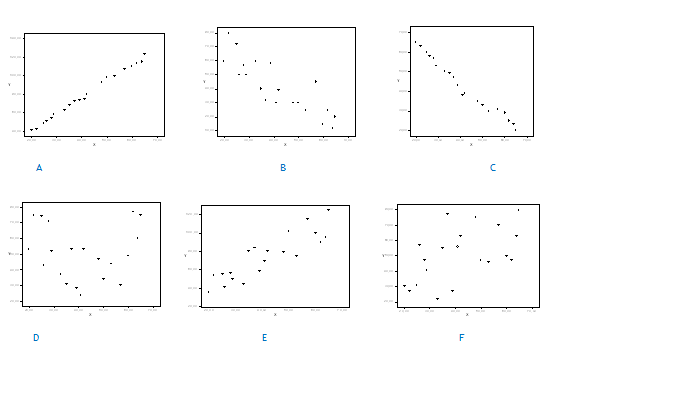
\includegraphics[width=1.10\textwidth]{correlaties.png}
  \captionof{figure}{Correlaties}
  \label{fig:correlaties}
  %\end{figure}
\end{exercise}

\begin{exercise}
  \label{ex:cats}
  Lees het databestand ``Cats.csv'' in. 
  \begin{enumerate}
    \item Voer een lineaire regressieanalyse uit op de variabelen Lichaamsgewicht (\texttt{Bwt}, afhankelijke variabele) en Gewicht hart (\texttt{Hwt}, onafhankelijke variabele).
    \item Maak een spreidingsdiagram van beide variabelen.
    \item Bereken en teken de regressielijn.
    \item Bereken de correlatie- en de determinatiecoëfficiënt.
    \item Geef een interpretatie van deze resultaten.
  \end{enumerate}
\end{exercise}

\begin{exercise}
  \label{ex:cats-per-geslacht}
  Gebruik dezelfde data als in vorige oefening.
  \begin{enumerate}
    \item Voer een lineaire regressieanalyse uit op de variabelen Lichaamsgewicht (Bwt) en Gewicht hart (Hwt) per geslacht.
    \item Maak een spreidingsdiagram van beide variabelen voor elk van de geslachten.
    \item Bereken en teken telkens de regressielijn.
    \item Bereken de correlatie- en de determinatiecoëfficiënt.
    \item Geef een interpretatie aan deze resultaten.
  \end{enumerate}
\end{exercise}

\begin{exercise}
  \label{ex:pizza}
  Lees het databestand ``Pizza.csv'' in.
  \begin{enumerate}
    \item Voer een volledige lineaire regressieanalyse uit op de variabelen Rating en CostPerSlice. Trek hieruit de juiste conclusies en ga deze ook grafisch na.
    \item Onderzoek een mogelijk verband tussen Rating en Neighbourhood. Welke methode kan je hiervoor gebruiken? Kan je de gegevens van Rating hiervoor in dezelfde vorm gebruiken?
    \item Geef een interpretatie aan deze resultaten.
    \item Stel de kruistabel grafisch voor met een staafdiagram.  Voorzie een legende.
  \end{enumerate}
\end{exercise}


%%%%%%%%%%%%%%%%%%%%%%%%%%%%%%%%%%%%%%%%%%%%%%%%%%%%%%



\section{Solutions to selected exercises}
\label{ssec:analyse-2-variabelen-oplossingen}

\paragraph{Oefening~\ref{ex:muziekwijn-analyse}}

$\chi^2 \approx 18,2792$, Cramér's $V \approx 0,1939$

\paragraph{Oefening~\ref{ex:chisq-survey}}

\begin{enumerate}
  \item \texttt{Exer}/\texttt{Smoke}: $\chi^2 = 5.4885$, $g = 12.59159$, $p = 0.4828422$
  \item \texttt{W.Hnd}/\texttt{Fold}: $\chi^2 = 1.581399$, $g = 5.9915$, $p = 0.454$
  \item \texttt{Sex}/\texttt{Smoke}: $\chi^2 = 3.554$, $g = 7.8147$, $p = 0.314$
  \item \texttt{Sex}/\texttt{W.Hnd}: $\chi^2 = 0.236$, $g = 3.8415$, $p = 0.627$
\end{enumerate}

\paragraph{Oefening~\ref{ex:chisq-aids2}} $\chi^2 = 1083.372914$, $g = 14.067140$, $p \approx 1.157 \times 10^{-229}$

\paragraph{Oefening~\ref{ex:chisq-digimeter}} $\chi^2 \approx 6.6997$ ($df = 6$), $g \approx 12.5916$, $p \approx 0.3495$


\paragraph{Oefening~\ref{oef:casus-akin2016-toets}}

Tabel~\ref{tab:akin2016-resultaten-ttoets} geeft een overzicht met voor elke datasetgrootte het beste en tweede beste persistentietype (op basis van het steekproefgemiddelde). De conclusie van~\textcite{Akin2016}, dat \emph{Realm} het performantste persistentietype is, blijft overeind, maar voor de kleine datasets is het verschil niet significant.

Merk op dat we hier niet expliciet vooraf een significantieniveau gekozen hebben. Voor $\alpha = 0,1$, $0,05$ of zelfs $0,01$, kunnen we echter dezelfde conclusie trekken.

\begin{table}
  \begin{center}
    \begin{tabular}{llll}
      \toprule
      \textbf{Grootte} & \textbf{Beste} & \textbf{2e beste} & \textbf{$p$-waarde} \\ \midrule
      Small            & Realm          & SharedPreferences & 0.1699     \\
      Medium           & Realm          & GreenDAO          & 0.0002506  \\
      Large            & Realm          & SQLite            & 0.0017     \\ \bottomrule
    \end{tabular}
  \end{center}
  \caption{Resultaten $t$-toets voor de beste en 2e beste persistentietype op basis van steekproefgemiddelde~\autocite{Akin2016}.}
  \label{tab:akin2016-resultaten-ttoets}
\end{table}

\paragraph{Oefening~\ref{ex:test-examen}}

\begin{itemize}
  \item $\beta_{0} \approx 0,6333$, $\beta_{1} \approx 0.9667$
  \item $Cov \approx 6,444$, $R \approx 0,9352$, $R^2 \approx 0,8747$
\end{itemize}

\paragraph{Oefening \ref{ex:cats} en \ref{ex:cats-per-geslacht}}

\begin{center}
  \begin{tabular}{lrrrrr}
  	\toprule
    \textbf{Selectie} & \textbf{$\beta_{0}$} & \textbf{$\beta_{1}$} & \textbf{$Cov$} & \textbf{$R$} & \textbf{$R^2$} \\
    \midrule
  	Hele dataset & -0.3511 & 4.0318 & 0.9496 & 0.8041 & 0.6466 \\
  	Female       &  2.9813 & 2.6364 & 0.1979 & 0.5320 & 0.2831 \\
  	Male         & -1.1768 & 4.3098 & 0.9419 & 0.7930 & 0.6289 \\
    \bottomrule
  \end{tabular}
\end{center}

